\documentclass[12pt]{report}
\usepackage[margin=1in]{geometry}
\usepackage{setspace} % for single/doublespacing commands
\usepackage{graphicx} % including graphics
\usepackage{sectsty} % sexy section headings
% \usepackage{pdfpages} % including multipage pdfs
\usepackage[export]{adjustbox} % for graphic frames and center
\usepackage{siunitx}
% \usepackage[numbered]{matlab-prettifier} % including matlab w/ syntax highlighting
% \usepackage[T1]{fontenc} % prettier matlab font
% \usepackage{xfrac} % more legible inline fractions (\sfrac)
\usepackage{lmodern} % font package for above
% \usepackage{multicol} % multiple columns
\usepackage[justification=centering]{caption} % figure captions (force centering)
% \usepackage{amsmath} % more math symbols and shit
\usepackage{enumitem} % add arguments for enumerate to change style
\usepackage[list=true]{subcaption} % subfigures with list of figure support
\usepackage{multirow}
% \usepackage{mathtools}
\usepackage{booktabs}
\usepackage{color}
\usepackage{ulem}
% \usepackage{blindtext}
\usepackage[numbers]{natbib}
\usepackage{contour}
\usepackage{tabularx}
% \usepackage{circuitikz} % drawing fancy shit
% \usepackage{cancel} % arrow and cross math cancel symbol
% \usepackage{lineno}
\usepackage{framed}
\usepackage{amssymb} % special math symbols
\usepackage{listings}
\usepackage{array}
% \usepackage{BOONDOX-cal} % fancy mathtype script
\usepackage{fancyhdr}
% \usepackage{flowchart}
\usepackage{color, colortbl}
\usepackage{tocloft}
\usepackage{url}
\usepackage{etoolbox}

\setlength{\parskip}{\baselineskip}%
\setlength{\parindent}{0pt}%
\setcounter{secnumdepth}{5}
\renewcommand{\bibname}{References}
\sisetup{output-exponent-marker=\ensuremath{\mathrm{e}}}
\newcommand{\PreserveBackslash}[1]{\let\temp=\\#1\let\\=\temp}
\newcolumntype{C}[1]{>{\PreserveBackslash\centering}p{#1}}
\newcolumntype{R}[1]{>{\PreserveBackslash\raggedleft}p{#1}}
\newcolumntype{L}[1]{>{\PreserveBackslash\raggedright}p{#1}}
\lstMakeShortInline[style=Matlab-editor]| % matlab inline escape character
\graphicspath{{images/}}
\renewcommand\thesection{\arabic{section}}
\renewcommand\labelitemi{---}
\lstset{numberstyle=\ttfamily\small\color{gray}}
% \renewcommand\linenumberfont{\ttfamily\small\color{gray}}
% \setlength\linenumbersep{6mm}
% \hbadness=99999  % or any number >=10000
\apptocmd{\sloppy}{\hbadness 10000\relax}{}{}
% \usetikzlibrary{arrows,calc,patterns,angles,quotes}
% \usetikzlibrary{shapes.geometric}
% \usetikzlibrary{decorations.pathmorphing,decorations.pathreplacing} % for snakes!
% \usetikzlibrary{positioning, circuits.logic.US}
\setlength{\cftbeforetoctitleskip}{-2em}
% \newcommand{\Lag}{\mathcal{L}} % lagrangian L
\allsectionsfont{\raggedright}

\begin{document}
\normalem
\begin{titlepage}
\flushleft
\doublespacing
\Large
\textsc{Test Document} \\
\normalsize
Trey Dufrene, Zack Johnson, David Orcutt, Alan Wallingford, Ryan Warner
\vfill
\center
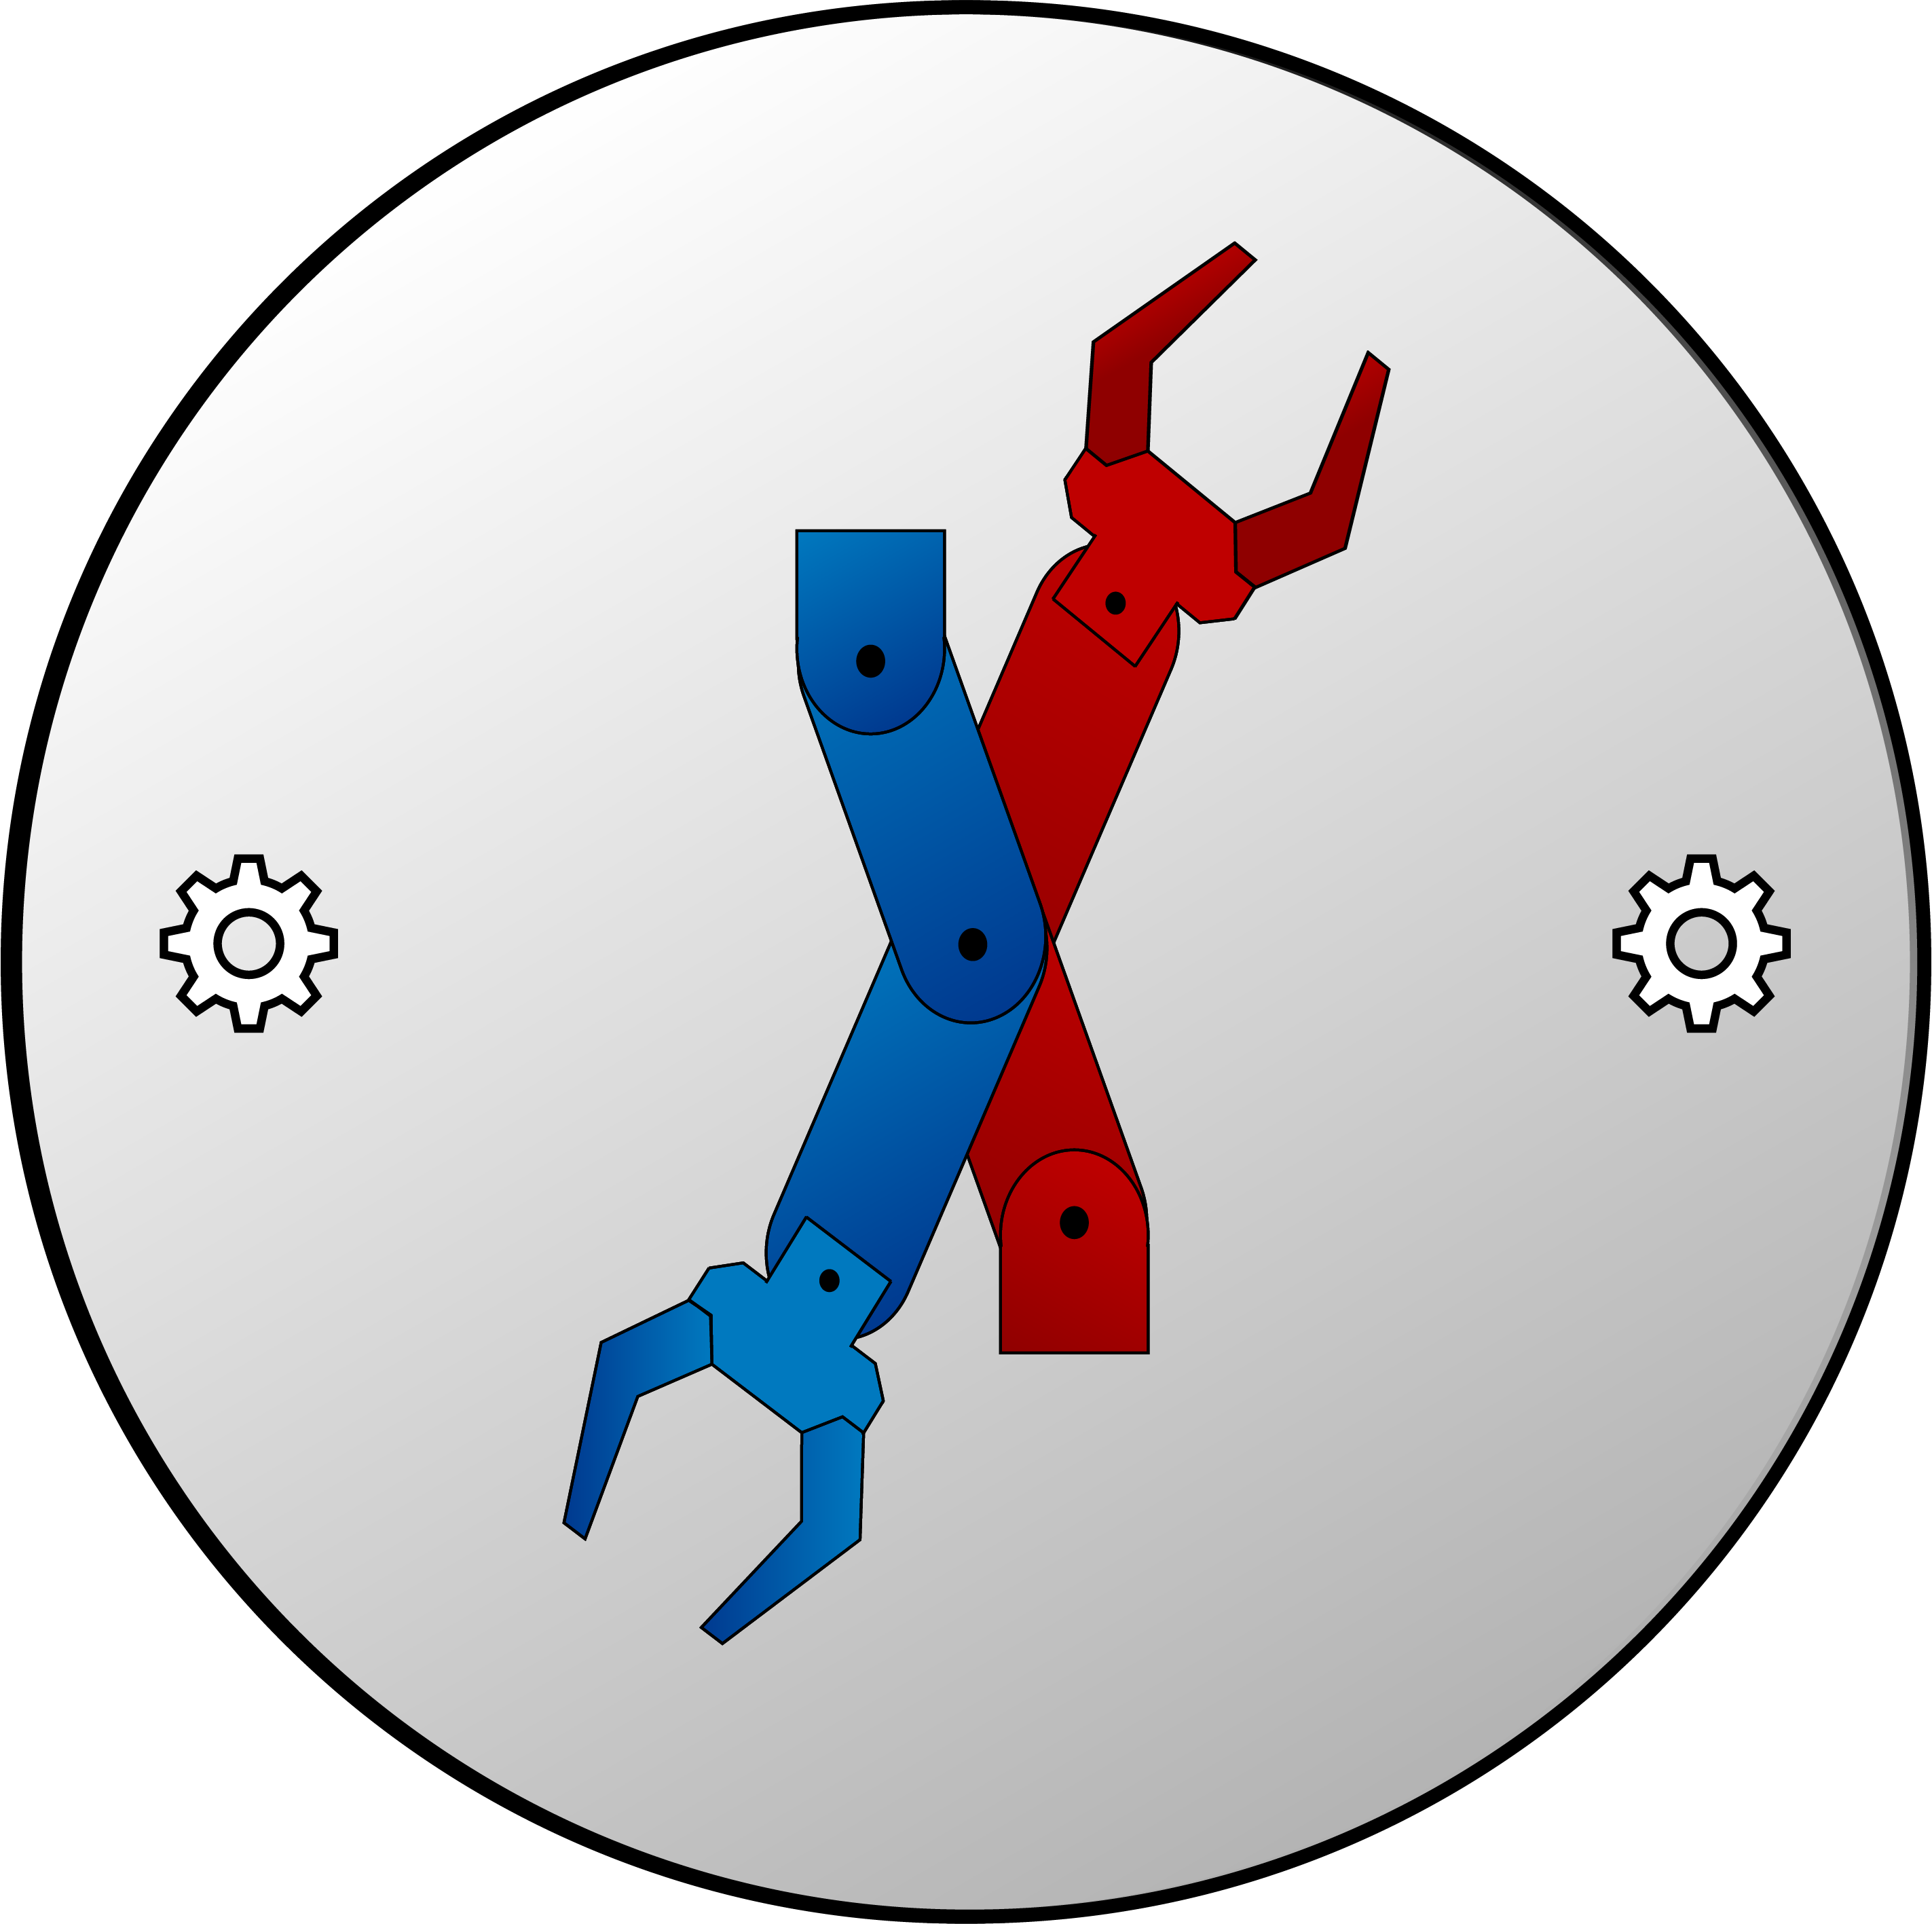
\includegraphics[width=.45\textwidth]{logo}
\vfill
\flushleft
ME 407 \\
Preliminary Design of Robotic Systems \\
Embry-Riddle Aeronautical University \\
\vspace{2ex}
\begin{minipage}[c]{.5\textwidth}
\flushleft

\includegraphics[width=.95\textwidth]{erau}
\end{minipage}%
\begin{minipage}[c]{.5\textwidth}
\flushright

\includegraphics[width=.8\textwidth]{text}
\end{minipage}
\end{titlepage}

\pagenumbering{roman}
% \begin{abstract}
  % Wordy words
% \end{abstract}
{\tableofcontents\let\clearpage\relax\listoffigures\let\clearpage\relax\listoftables}
\clearpage
\newpage

% \section*{List Of Acronyms and Abbreviations}

% \begin{tabular}{rl}
%   $G$~:&Center of gravity of the bar \\
%   $\ell_0$~:& Spring unstretched length  \\
%   $\delta$~:& Spring deflection \\
%   $k$~:& Spring constant \\
%   $h_{b}$~:& Distance to bar ($G$) from datum \\
%   $F_s$~:& Force onto bar due to spring\\
%   $A_{n}$~:& Pin reaction in $\theta$ direction\\
%   $A_{t}$~:& Pin reaction in tangential direction \\
%   $\vec{v}_G$~:& Velocity of bar center of gravity\\
%   $\ddot{\theta}$~:& Angular velocity of spring \\
%   $\ddot{\phi}$~:& Angular velocity of bar\\
%   $\ddot{\ell}_s$~:& Radial acceleration of spring \\
% \end{tabular}
% \normalsize
% \flushleft
% \singlespacing
% \newpage

\pagenumbering{arabic}

\section{Introduction}
\section{Design Requirements}
\subsection{Hardware}
\subsubsection{The system shall cost the end-user no more than \$1000.}
\subsubsection{The system shall be fully dexterous without being kinematically redundant.}
\subsubsection{The system end effector shall maintain a positional accuracy magnitude of \(\pm 1\) mm and an orientation accuracy of \(\pm 5^{\circ}\) eigen angle from the base frame.}
\subsubsection{The system end effector shall maintain a pose repeatability magnitude between 0.1—1.5 mm for the position and \(\pm 4^{\circ}\) eigen angle from the base frame for the orientation.}
\subsubsection{The system’s reachable workspace shall be a hemisphere with a radius of 300-700 mm.}
\subsubsection{The system’s dexterous workspace shall be a hemisphere within the workspace with a difference between the outer and inner radii of 280 mm.}
\subsubsection{The system shall have a removable end effector capable of picking and placing a low-odor chisel tip Expo dry erase marker.}
This creates a robot capable of performing a variety of basic tasks, which enhances its educational value.
\begin{enumerate}[label=\thesubsubsection\alph*.,leftmargin=3cm,font=\itshape]
  \item \textit{The system will use a parallel gripper (purchased or 3D-Printed).} \\
  This will be sufficient to perform pick and place operation on an Expo dry erase marker.
  \item \textit{The end effector will attach to the manipulator using screws.}\\
  This connection point will be standardized and will support many different configurations of screw positions. This allows for various grippers or custom end effectors to be implemented.
\end{enumerate}


\subsubsection{The system shall be able to write with a low-odor chisel tip Expo dry erase marker.}
\begin{enumerate}[label=\thesubsubsection\alph*.,leftmargin=3cm,font=\itshape]
  \item \textit{The end effector will be capable of holding the marker still while moving.}\\
  In order to be reliable when drawing, the marker should not move while being manipulated by the robot.
  \item \textit{The end user will be able to select two points at which the robot will follow a trajectory between.} \\
  This keeps the marker on the surface while moving to enable the robot to draw.
\end{enumerate}

\subsection{Software}
\subsubsection{The system shall be open source.}
\subsubsection{The system shall be capable of operating given only desired end effector cartesian coordinates specified with respect to the base frame.}
\end{document}
